\documentclass[11pt,a4paper]{article}
\usepackage[utf8]{inputenc}
\usepackage[a4paper, margin=0.3in]{geometry}
\usepackage{authblk}
\usepackage{wrapfig}
\usepackage{graphicx}
\graphicspath{ {./images/} }


\title{ENPM808X Mid-Term Proposal}
\author[*]{Aman Sharma}
\author[*]{Daniel}
\author[*]{Shantanu Parab}
\affil[*]{Professional Master's in Robotics, University of Maryland}

\date{October 2022}

\begin{document}

\maketitle
\section*{Introduction}
\begin{wrapfigure}{r}{0.18\textwidth}
    \centering
    % \caption{Implementation Diagram}
    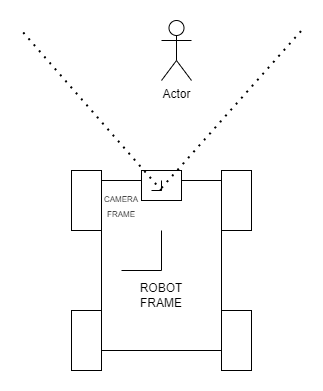
\includegraphics[width=4cm, height=4cm]{images/REPORT DIAGRAM.png}
\end{wrapfigure}
ACME Robotics is planning to build an autonomous robot that can maneuver through a field. The robot has to detect humans as obstacles and make informative decisions to travel through the area without collision. 
This project's scope is to develop software for detecting humans and tracking them to integrate with the robot. The input stream of images will be using a monocular camera. 

\section*{Implementation}
The module will be integrated into the robot in such a way that it can provide the relative position of the human obstacle with respect to the robot's frame of reference. The camera is mounted to the front of the robot.
\section*{Development Process}
We will be following the \textbf{Agile Iterative Process} along with \textbf{Test Driven Development}. The team will work in weekly iterations and keep a  track of the backlog in a backlog chart. The commits at the end of the day will be built overnight proceeded by a daily meeting to discuss the impediments, reflect on the previous build and decide future deadlines. We will be using Git Version Control to keep a track of the progress. The unit test will be created to check the functionality of the code. We will be using best practices from TDD to minimize the errors and best coding and documentation to provide documentation.

\section*{Resources}
\textbf{Algorithm} YOLO OpenSource\\
\textbf{Libraries} OpenCV OpenSource\\
\textbf{Programming Language} C++ \\
\textbf{Build System} Cmake \\

\section{Algorithm}

\section*{Risks and Mitigation}
\subsection*{Risks}
\begin{itemize}
  \item Poor Quality video.
  \item Modeling Biases
  \item Ambient Light
  \item Incompatible processing and frame speed
\end{itemize}
\subsection*{Mitigation}
\begin{itemize}
  \item Get proper video quality
\item Check for compatible processing
\item Have a light setup to illuminate the area under observation
\item Get a bigger data set.

\end{itemize}

\section*{Deliverable}
We will provide a program that can provide the coordinates of a human obstacle with respect to a robot frame.
These coordinates will be based on few assumption defined in the proposal and should be considered as estimates.
Precise outcomes can be obtained by changing these assumptions to actual real time parameters.
\end{document}
